\secrel{Структура компилятора}\label{compiler}\secdown

\secrel{Термины}

\begin{description}
\item[исходный код], исходник: текстовое представление программы,
предназначенное для чтения и написания человеком. Формат определяется
синтаксисом используемого языка программирования или описания данных 
\item[лексер] \ref{lexer}\ программный компонент, выполняющий выделение 
синтаксических элементов (токенов) из входного потока символов.
\item[токен] объект, содержащий выделенный из исходного кода текст,
имя файла/строку/столбец исходника, маркер типа данных (число, строка, оператор),
и т.п.
\item[парсер] \ref{parser}\ компонент, выполняющий анализ структуры текстового файла данных,
с учетом вложенных скобок, синтаксических блоков типа begin/end, условных конструкций,
описаний числовых матриц и векторов, и т.п.
\item[AST] [A]bstract [S]yntax [T]ree, абстрактное синтаксическое дерево\\
вложенная структура данных, состоящая из синтаксических объектов: 
терминалы (целые, строки, символы,..) и нетерминалы (операторы ссылающиеся на операнды,
блоки кода содержащие списки операцией,..). AST хранит информацию о вложенности конструкций,
порядке вычислений выражений, подчиненности элементов и т.п.

\noindent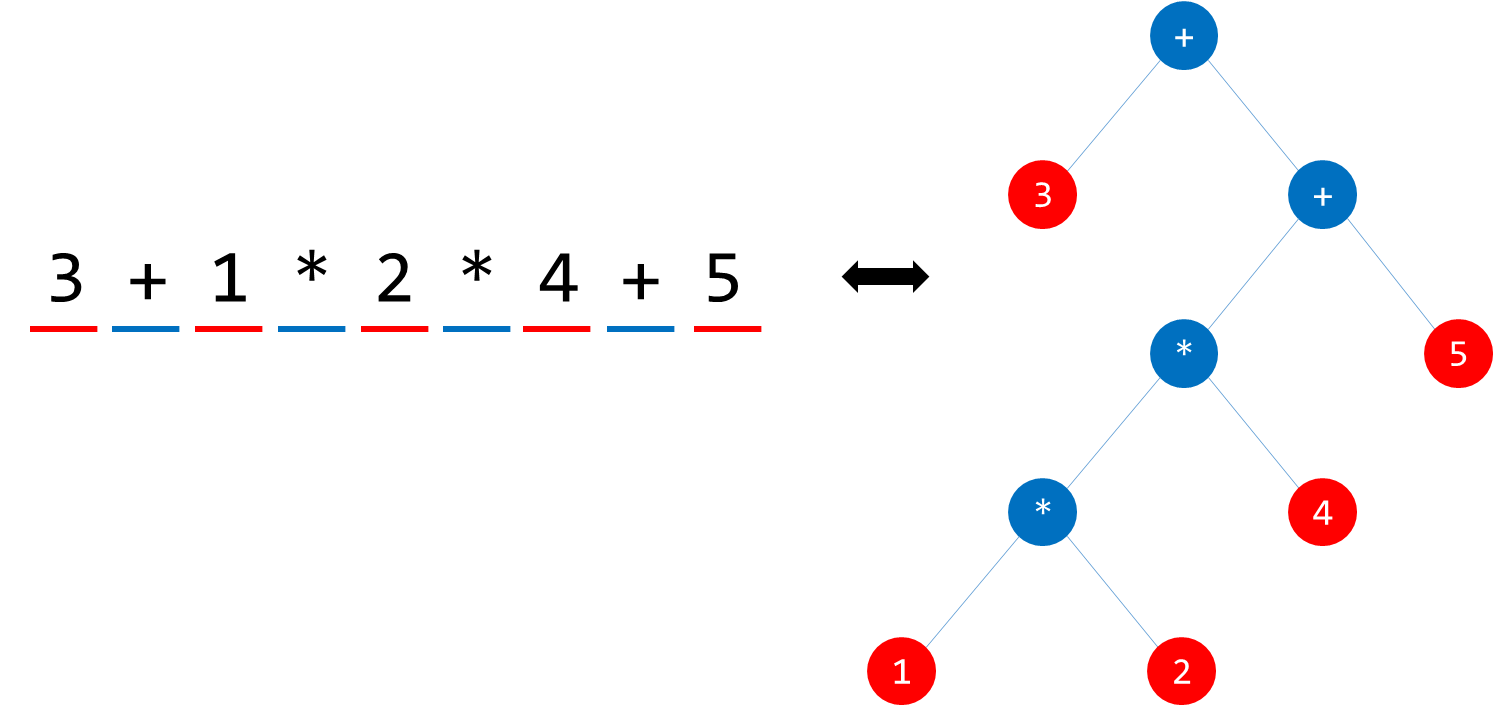
\includegraphics[height=0.5\textheight]{fig/ast.png}

\item[SSA] \ref{ssa}\ \href{https://ru.wikipedia.org/wiki/SSA}{[S]ingle [S]tate
[A]ssignment}, 
однократное назначение: промежуточное представление, в котором каждой переменной 
значение присваивается лишь единожды. Переменные исходной программы разбиваются 
на версии, обычно с помощью добавления суффикса, таким образом, что каждое 
присваивание осуществляется уникальной версии переменной.
В SSA используются \term{машинно-независимые трехадресные команды} 
абстрактной виртуальной машины. 

  
\end{description}

\secrel{Структура типового компилятора}

\includegraphics[height=0.9\textheight]{fig/compiler1.png}

\pagebreak
\includegraphics[width=0.95\textwidth]{fig/compiler2.png}

\secrel{Архитектура LLVM}
\noindent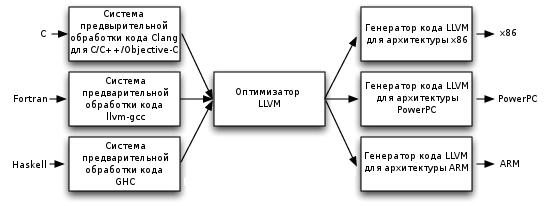
\includegraphics[width=\textwidth]{fig/llvm.png}

\secup
